\textbf{Цель работы:} определить горизонтальную составляющую магнитного
поля Земли и установить количественное соотношение между единицами
электрического тока в системах СИ и СГС.
\\\indent
\textbf{Оборудование:} магнитометр, осветитель со шкалой, источ­
ник питания, вольтметр, электромагнитный переключатель, конденсатор,
намагниченный стержень, прибор для определения периода крутильных
колебаний, секундомер, рулетка, штангенциркуль. 
\section*{Экспериментальная установка}
\begin{figure}
    \centering
    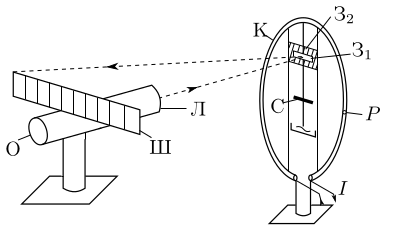
\includegraphics[width=10cm]{setup.png}
    \caption{Схема установки}
\end{figure}
Магнитометр состоит из нескольких последовательно соединённых круговых витков К. В центре кольца К радиусом $R$ на нити подвешена короткая магнитная стрелка С. В отсутствие других магнитных полей стрелка располагается по направлению горизонтальной составляющей земного магнитного поля $B_0$. 
\\\indentПрибор настраивают с помощью световых зайчиков, отражённых от двух зеркал: З1, прикреплённого к стрелке, и З2, расположенного в плоскости кольца К и жёстко связанного с ним. Оба зеркала освещаются одним и тем же осветителем О.
\\\indentПри появлении дополнительного горизонтального магнитного поля $B_{\perp}$ стрелка C установится по равнодействующей обоих полей $B_{\sum}$. 
В нашей установке дополнительное поле может быть создано
либо малым ферромагнитным стержнем, расположенным на кольце на
его горизонтальном диаметре ($B_1$), либо током, проходящим по кольцу
($B_2$). В обоих случаях дополнительное поле можно считать однородным,
так как размеры стрелки много меньше радиуса кольца.
\begin{align}
    B_1 = \frac{\mu_0}{4\pi}\frac{m}{R^3}, \hspace{1cm} B_2 = N\frac{\mu_0 I}{2R}
\end{align}
где $m$ - магнитный момент стержня; $I$ - сила тока в кольце; $N$ - число витков в кольце.\\\indent
Поля $B_1, B_2$ и угол отклонения стрелки $\varphi$ связаны соотношением 
\begin{equation}
    B_{\perp} = B_0 \cdot \tg{\varphi}
\end{equation}
Поле намагниченного стержня вдали от него можно считать:
\begin{equation}
\bar{B}(\bar{r}) = \frac{\mu_0}{4\pi}\left (2\frac{(\bar{m}\cdot \bar{r})\bar{r}}{r^5} - \frac{\bar{m}}{r^3}\right )
\end{equation}

\subsection*{Определение горизонтальной составляющей магнитного поля Земли}
\indent В отверстие Р устанавливается намагниченный стержень. Стрелка отклонится на угол $\varphi_1$, что 
\begin{equation}
    \tg{\varphi_1} = \frac{x_1}{2L}
\end{equation}
\indent Исключим из выражения $\bar{m}$, измерив период крутильных колебаний стержня в поле Земли.
\begin{align}
    M_{\text{мех}} &= |\bar{m}\times \bar{B}| \approx \bar{m}B_0 \alpha\\
    J\ddot{\alpha} + m\B_0\alpha &= 0\\
    T &= 2\pi\sqrt{\frac{J}{m B_0}}\\
    J &= m\left ( \frac{l^2}{12} + \frac{r^2}{4}\right )
\end{align}
Из этого всего получаем выражение для горизонтальной составляющей магнитного поля Земли:
\begin{equation}
    B_0 = \frac{2\pi}{TR}\sqrt{\frac{\mu_0 I L}{2\pi R x_1}}
\end{equation}
\subsection*{Определение электродинамической постоянной}
\indent Ток в цепи кольца можно измерить двумя независимыми способами:
по магнитному действию тока на стрелку магнитометра и по заряду,
протекающему через цепь в единицу времени.По отношению результатов этих измерений
можно определить электродинамическую постоянную $c$.
По формулам 1-2 получаем:
\begin{equation}
    I = \frac{2B_0R}{\mu_0 N}\tg{\varphi_2} \hspace{1cm} [\text{СИ}]
\end{equation}
\indent Второй способ: разрядим конденсатор ($C$), заряженный до $U$, через витки, то через них пройдет заряд $q = CU$. Если $\nu$ раз в секунду заряжать и разряжать, то средний ток будет: $I = CU\nu [\text{абс}]$. 
Тогда определяем значение электродинамической постоянной как:
\begin{equation}
    c\left [\frac{\text{м}}{\text{с}}\right ] = \frac{1}{10}\frac{I_{[\text{СГС}]}}{I _{[\text{СИ}]}}
\end{equation}
